\documentclass[12pt,a4paper]{article}
\usepackage{ctex}
\usepackage{amsmath,amssymb,amsthm}
\usepackage{geometry}
\geometry{margin=2.4cm}
\usepackage{tikz}
\newtheorem*{model}{模型}
\newtheorem*{proofdemo}{证明}

\begin{document}
	\title{1 初一}
	\author{}
	\date{}
	\maketitle
	
	\section{猪蹄模型（M型）}
	\begin{model}
		已知 $AB \parallel CD$，拐点 $E$ 在两条平行线之间，连接 $BE,DE$。
		结论：$\angle BED = \angle ABE + \angle CDE$。
	\end{model}
	
	\begin{center}
		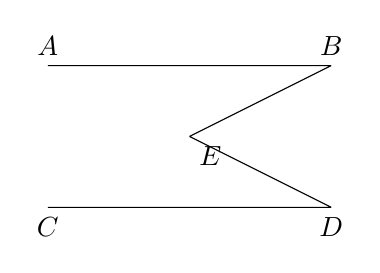
\begin{tikzpicture}[scale=0.9]
			\coordinate (A) at (-2,1);
			\coordinate (B) at (2,1);
			\coordinate (E) at (0,0);
			\coordinate (C) at (-2,-1);
			\coordinate (D) at (2,-1);
			\draw (A)--(B) (B)--(E) (E)--(D) (D)--(C);
			\node[above] at (A) {$A$};
			\node[above] at (B) {$B$};
			\node[below right] at (E) {$E$};
			\node[below] at (C) {$C$};
			\node[below] at (D) {$D$};
		\end{tikzpicture}
	\end{center}
	
	\begin{proofdemo}
		已知 $AB\parallel CD$，过点 $E$ 作 $EG\parallel AB$。
		
		由两直线平行，内错角相等，可得
		$\angle ABE=\angle BEG$。
		
		又因为 $AB$ 平行于 $CD$，$EG$ 平行于 $AB$，根据平行公理的推论，有 $EG$ 平行于 $CD$，
		于是可得 $\angle CDE=\angle DEG$。
		
		将上面两个等式相加，得到 $\angle ABE+\angle CDE=\angle BEG+\angle DEG$，
		而 $\angle BEG+\angle DEG=\angle BED$，
		因此 $\angle BED=\angle ABE+\angle CDE$。
		
		证毕。
	\end{proofdemo}
	
	\clearpage
	\section{铅笔头模型}
	\begin{model}
		已知 $AB \parallel CD$，拐点 $E$ 在平行线外侧向外弯折，连接 $BE,DE$。
		结论：$\angle ABE+\angle BED+\angle EDC=360^\circ$。
	\end{model}
	
	\begin{center}
		\begin{tikzpicture}[scale=0.9]
			\coordinate (A) at (0,2);
			\coordinate (B) at (5,2);
			\coordinate (E) at (6,0);
			\coordinate (C) at (0,-2);
			\coordinate (D) at (5,-2);
			\draw (A)--(B) (B)--(E) (E)--(D) (D)--(C);
			\node[above] at (A) {$A$};
			\node[above] at (B) {$B$};
			\node[right] at (E) {$E$};
			\node[below] at (C) {$C$};
			\node[below] at (D) {$D$};
		\end{tikzpicture}
	\end{center}
	
	\begin{proofdemo}
		已知 $AB\parallel CD$，过点 $E$ 作 $EG\parallel AB$。
		
		由两直线平行，同旁内角互补，可得
		$\angle ABE+\angle BEG=180^\circ$。
		
		又因为 $AB$ 平行于 $CD$，$EG$ 平行于 $AB$，根据平行公理的推论，有 $EG$ 平行于 $CD$，
		于是可得 $\angle EDC+\angle DEG=180^\circ$。
		
		将上面两个等式相加，得到 $\angle ABE+\angle BEG+\angle DEG+\angle EDC=360^\circ$，
		而 $\angle BEG+\angle DEG=\angle BED$，
		因此 $\angle ABE+\angle BED+\angle EDC=360^\circ$。
		
		证毕。
	\end{proofdemo}
	
	\clearpage
	\section{鹰嘴（钩子/倒钩）模型}
	\begin{model}
		已知 $AB \parallel CD$，拐点 $E$ 在平行线外侧，连接 $BE,DE$。
		结论：$\angle BED=\angle ABE-\angle CDE$。
	\end{model}
	
	\begin{center}
		\begin{tikzpicture}[scale=0.9]
			\coordinate (A) at (-2,1);
			\coordinate (B) at (2,1);
			\coordinate (E) at (3,0);
			\coordinate (C) at (-2,-1);
			\coordinate (D) at (1,-1);
			\draw (A)--(B) (B)--(E) (E)--(D) (D)--(C);
			\node[above] at (A) {$A$};
			\node[above] at (B) {$B$};
			\node[right] at (E) {$E$};
			\node[below] at (C) {$C$};
			\node[below] at (D) {$D$};
		\end{tikzpicture}
	\end{center}
	
	\begin{proofdemo}
		已知 $AB\parallel CD$，过点 $E$ 作 $EG\parallel AB$。
		
		由两直线平行，内错角相等，可得
		$\angle ABE=\angle BEG$。
		
		又因为 $AB$ 平行于 $CD$，$EG$ 平行于 $AB$，根据平行公理的推论，有 $EG$ 平行于 $CD$，
		于是可得 $\angle CDE=\angle DEG$。
		
		将上面两个等式相减，得到 $\angle ABE-\angle CDE=\angle BEG-\angle DEG$，
		而 $\angle BEG-\angle DEG=\angle BED$，
		因此 $\angle BED=\angle ABE-\angle CDE$。
		
		证毕。
	\end{proofdemo}
	
	\clearpage
	\section{锯齿模型（多拐点折线模型）}
	\begin{model}
		已知 $AB \parallel CD$，图中有多个交替方向的拐点。
		结论：所有朝左侧的尖角之和等于所有朝右侧的尖角之和。
		以双拐点 $E,F$ 为例：$\angle ABE+\angle EFD=\angle BEF+\angle FDC$。
	\end{model}
	
	\begin{center}
		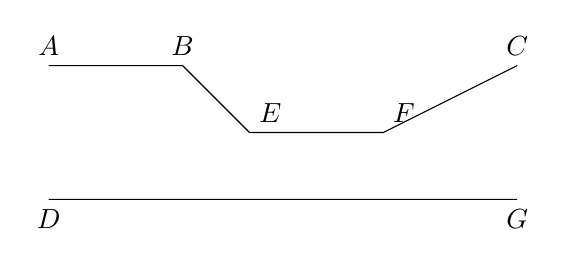
\begin{tikzpicture}[scale=0.85]
			\coordinate (A) at (-3,1);
			\coordinate (B) at (-1,1);
			\coordinate (E) at (0,0);
			\coordinate (F) at (2,0);
			\coordinate (C) at (4,1);
			\coordinate (D) at (-3,-1);
			\coordinate (G) at (4,-1);
			\draw (A)--(B) (B)--(E) (E)--(F) (F)--(C) (D)--(G);
			\node[above] at (A) {$A$};
			\node[above] at (B) {$B$};
			\node[above] at (C) {$C$};
			\node[below] at (D) {$D$};
			\node[below] at (G) {$G$};
			\node[above right] at (E) {$E$};
			\node[above right] at (F) {$F$};
		\end{tikzpicture}
	\end{center}
	
	\begin{proofdemo}
		已知 $AB\parallel CD$，分别过点 $E,F$ 作 $EG\parallel AB$，$FH\parallel AB$。
		
		由两直线平行，内错角相等，可得
		$\angle ABE=\angle BEG,\ \angle GEF=\angle EFH,\ \angle HFC=\angle FCD$。
		
		整理角度等量关系，把朝左的角度放在一侧，朝右的角度放在另一侧，
		因此朝左侧角度总和等于朝右侧角度总和。
		
		证毕。
	\end{proofdemo}
	
\end{document}
